% THIS IS SIGPROC-SP.TEX - VERSION 3.1
% WORKS WITH V3.2SP OF ACM_PROC_ARTICLE-SP.CLS
% APRIL 2009
%
% It is an example file showing how to use the 'acm_proc_article-sp.cls' V3.2SP
% LaTeX2e document class file for Conference Proceedings submissions.
% ----------------------------------------------------------------------------------------------------------------
% This .tex file (and associated .cls V3.2SP) *DOES NOT* produce:
%       1) The Permission Statement
%       2) The Conference (location) Info information
%       3) The Copyright Line with ACM data
%       4) Page numbering
% ---------------------------------------------------------------------------------------------------------------
% It is an example which *does* use the .bib file (from which the .bbl file
% is produced).
% REMEMBER HOWEVER: After having produced the .bbl file,
% and prior to final submission,
% you need to 'insert'  your .bbl file into your source .tex file so as to provide
% ONE 'self-contained' source file.
%
% Questions regarding SIGS should be sent to
% Adrienne Griscti ---> griscti@acm.org
%
% Questions/suggestions regarding the guidelines, .tex and .cls files, etc. to
% Gerald Murray ---> murray@hq.acm.org
%
% For tracking purposes - this is V3.1SP - APRIL 2009

\documentclass{acm_proc_article-sp}

\usepackage[utf8]{inputenc}
\usepackage[brazilian]{babel}
\usepackage{color}
\usepackage{listings}
\usepackage{textcomp}
%\usepackage{algorithm2e}
%\hyphenation{po-de-ría-mos}
\newcommand{\todo}[1]{\textcolor[rgb]{1.00,0.00,0.00}{\bf \uppercase{#1}}}

\begin{document}

\title{Uma nova técnica para criação de videoconferências em dispositivos móveis Android}
%
% You need the command \numberofauthors to handle the 'placement
% and alignment' of the authors beneath the title.
%
% For aesthetic reasons, we recommend 'three authors at a time'
% i.e. three 'name/affiliation blocks' be placed beneath the title.
%
% NOTE: You are NOT restricted in how many 'rows' of
% "name/affiliations" may appear. We just ask that you restrict
% the number of 'columns' to three.
%
% Because of the available 'opening page real-estate'
% we ask you to refrain from putting more than six authors
% (two rows with three columns) beneath the article title.
% More than six makes the first-page appear very cluttered indeed.
%
% Use the \alignauthor commands to handle the names
% and affiliations for an 'aesthetic maximum' of six authors.
% Add names, affiliations, addresses for
% the seventh etc. author(s) as the argument for the
% \additionalauthors command.
% These 'additional authors' will be output/set for you
% without further effort on your part as the last section in
% the body of your article BEFORE References or any Appendices.

\numberofauthors{4} %  in this sample file, there are a *total*
% of EIGHT authors. SIX appear on the 'first-page' (for formatting
% reasons) and the remaining two appear in the \additionalauthors section.
%
\author{
% You can go ahead and credit any number of authors here,
% e.g. one 'row of three' or two rows (consisting of one row of three
% and a second row of one, two or three).
%
% The command \alignauthor (no curly braces needed) should
% precede each author name, affiliation/snail-mail address and
% e-mail address. Additionally, tag each line of
% affiliation/address with \affaddr, and tag the
% e-mail address with \email.
%
% 1st. author
%\alignauthor
Giancarlo Rampanelli, 
Felipe Cecagno,
André Schulz,
Valter Roesler\\
%       \affaddr{Laboratório do PRAV}\\
       \affaddr{Instituto de Informática}\\
       \affaddr{Universidade Federal do Rio Grande do Sul}\\
       \affaddr{Porto Alegre, Rio Grande do Sul, Brasil}\\
       \email{\{grampanelli, fcecagno, aschulz, roesler\}@inf.ufrgs.br}
}
\date{15 de maio de 2011}

\maketitle
\begin{resumo}
  Este artigo tem o objetivo de apresentar uma nova estratégia para criação de videoconferências em dispositivos móveis com sistema operacional Android. É apresentado um estudo sobre as classes multimídia padrão do kit de desenvolvimento de software do Android, detalhando as limitações que dificultam o desenvolvimento de sistemas multimídia em tempo real sem a utilização de bibliotecas externas. Várias soluções propostas em trabalhos anteriores são comparadas, ressaltando prós e contras, e conduzindo a necessidade da utilização de uma nova estratégia, detalhada neste artigo, que é baseada principalmente em bibliotecas alternativas. A ideia proposta é então validada num sistema Android real, mostrando suas vantagens.
\end{resumo}

\begin{abstract}
  This paper aims to present a novel strategy for implementation of real-time interactive multimedia systems on Android-powered mobile devices. We will present a study about the standard multimedia classes of Android’s software development kit, detailing the limitations that hinder the development of real time multimedia systems without using external libraries. Some alternative solutions proposed in previous works will be presented, driving to the need of using a new strategy, detailed in this article, which is based primarily on alternative libraries. The proposed idea is then validated in a real Android system, showing its advantages.
\end{abstract}

% http://www.acm.org/about/class/ccs98-html
% A category with the (minimum) three required fields
%\category{}{Peer-to-peer multimedia systems and streaming}{}
%\category{}{Software development using multimedia techniques}{}
%\category{H.4}{Information Systems Applications}{Miscellaneous}


\category{C.3}{Special-purpose and application-based systems}{Real-time and embedded systems}
\category{J.7}{Computers in other systems}{Real time}
\category{I.6}{Simulation and modeling}{Applications}
\category{H.4}{Information systems applications}{Communications Applications}{Computer conferencing, teleconferencing, and videoconferencing}

\terms{Design, Experimentation}

\keywords{Interação multimídia de tempo real, Vídeo, JNI}

\section{Introdução}

Sistemas de transmissão de vídeo interativo em tempo real são complexos de serem desenvolvidos, uma vez que, além da necessidade de áudio e de vídeo serem capturados, transmitidos, recebidos e exibidos de forma contínua por todos os participantes, é necessário que esse processo ocorra com baixa latência. Se o intervalo de tempo entre a captura e a exibição nos pontos remotos ultrapassar 400 milissegundos, o resultado pode ser uma interação altamente frustrante~\cite{kurose_2001}.

É um desafio desenvolver com qualidade tais sistemas pois as redes comerciais atuais, em geral, possuem largura de banda restrita. O desafio se torna ainda maior na área de dispositivos móveis, que tipicamente possuem hardware limitado, o que torna a manipulação de vídeo um ponto crítico do sistema. Além disso, smartphones e tablets se conectam à Internet através de redes 3G ou Wi-Fi, ambas caracterizadas por altas taxas de perda de pacotes e baixas velocidades~\cite{huynh-thu_2008}. 

Um sistema de interação por vídeo pode ser dividido em dois módulos:
\begin{itemize}
 \item Um módulo origem, composto de:
 \begin{itemize}
  \item um sub-módulo que captura áudio e vídeo não comprimidos do microfone e da câmera, respectivamente;
  \item um sub-módulo que codifica áudio e vídeo;
  \item um sub-módulo que envia pela rede os dados codificados;
 \end{itemize}
 \item Um módulo destino, composto de:
 \begin{itemize}
  \item um sub-módulo que recebe da rede dados de áudio e vídeo codificados;
  \item um sub-módulo que decodifica áudio e vídeo;
  \item um sub-módulo que exibe os dados decodificados para o usuário.
 \end{itemize}
\end{itemize}

Neste trabalho será apresentada uma nova estratégia para criação de sistemas de videoconferência em dispositivos móveis com sistema operacional Android. Para justificar as escolhas feitas e a utilização de bibliotecas alternativas, primeiramente será feita uma análise da Software Development Kit (Kit de Desenvolvimento de Software - SDK) do Android para multimídia, seguida de uma comparação de possíveis estratégias propostas por trabalhos anteriores para desenvolvimento de sistemas de interação por vídeo em tempo real com a utilização apenas das classes padrão do Android, e de suas limitações. Por fim, para validar a estratégia, são realizadas implementações e os devidos resultados são apresentados.

\section{Análise da SDK do Android para multimídia}

O Android é um sistema operacional de código aberto voltado principalmente para dispositivos móveis, desenvolvido numa colaboração entre Google e outros membros da Open Handset Alliance, e baseado no núcleo do Linux. Em comparação com outros sistemas operacionais existentes para dispositivos móveis, o Android é caracterizado por aplicações de vídeo mais simples. Isso se deve às limitações das APIs disponibilizadas pelo Android para programação de aplicativos de vídeo e, alternativamente, à grande complexidade para criar tais aplicativos utilizando APIs alternativas. A dificuldade de se encontrar bons aplicativos de vídeo para Android se torna ainda mais marcante na área de vídeo interativo.

Aplicativos para Android são escritos na linguagem de programação Java e executam sobre a máquina virtual Dalvik. O desenvolvimento de aplicativos é feito com o auxílio da SDK do Android, que fornece, além das plataformas para compilação, uma variedade de ferramentas úteis no desenvolvimento, como depuradores de código e emuladores~\cite{ableson_2009}. 

É possível ainda desenvolver módulos de aplicativos nas linguagens C e C++, visto que o Android executa sobre o núcleo do Linux \todo{(FU et al., 2010)}. Para isso, é necessário utilizar a Native Development Kit (Kit de Desenvolvimento Nativo - NDK) para Android. Entretanto, não é possível executar um aplicativo totalmente desenvolvido utilizando a NDK - é necessário que o ponto de partida do aplicativo seja escrito em Java. A interação entre o código Java e o código nativo é feita através da JNI (Java Native Interface), interface que permite que um código que está executando em uma máquina virtual interaja com um código nativo \todo{(FU et al., 2010)}.

As classes de referência da SDK do Android que podem ser importantes para o desenvolvimento de um sistema de interação através de áudio e vídeo podem ser classificadas como segue:
\begin{itemize}
 \item Para o módulo de origem: MediaRecorder, Camera e AudioRecord;
 \item Para o módulo de destino: MediaPlayer e AudioTrack.
\end{itemize}

Existem outras classes relacionadas, porém estas apresentam pequenas extensões ou encapsulamentos das classes acima, sem importância para este trabalho. Também existem classes relacionadas ao envio e recebimento de dados genéricos pela rede que podem ser utilizadas em conjunto com as classes acima. A seguir as classes supracitadas serão detalhadas, e com base nas características de cada uma serão apresentadas estratégias de desenvolvimento de um sistema de vídeo interativo bem como suas limitações.

\lstset{
    language=java,
    basicstyle=\scriptsize,
    upquote=true,
%    aboveskip={1.5\baselineskip},
    columns=fullflexible,
    showstringspaces=false,
    extendedchars=true,
    breaklines=true,
    showtabs=false,
    showspaces=false,
    showstringspaces=false,
    identifierstyle=\ttfamily,
    keywordstyle=\color[rgb]{0,0,1},
    commentstyle=\color[rgb]{0.133,0.545,0.133},
    stringstyle=\color[rgb]{0.627,0.126,0.941},
}

\subsection{Classe MediaRecorder}
A classe MediaRecorder realiza a captura de áudio e vídeo (através do microfone e da câmera) e codifica os dados utilizando o hardware disponível no aparelho. Os dados codificados podem ser salvos em arquivo ou transmitidos pela rede por meio de sockets. A classe também permite a exibição de uma pré-visualização local da captura para o usuário. A utilização do MediaRecorder acontece da seguinte forma~\ref{developers_android}:
\begin{enumerate}
 \item Declarar uma instância da classe
  \begin{lstlisting}
MediaRecorder mMediaRecorder = new MediaRecorder();
  \end{lstlisting}
 \item Escolher as fontes de áudio e vídeo:
  \begin{lstlisting}
mMediaRecorder.setAudioSource(<fonte_de_audio>);
mMediaRecorder.setVideoSource(<fonte_de_video>);
  \end{lstlisting}
 \item Escolher o destino (arquivo ou socket)
  \begin{lstlisting}
mMediaRecorder.setOutputFile(<destino>);
  \end{lstlisting}
 \item Iniciar a captura:
  \begin{lstlisting}
mMediaRecorder.prepare();
mMediaRecorder.start();
  \end{lstlisting}
 \item Exibir o preview da captura:
  \begin{lstlisting}
mMediaRecorder.setPreviewDisplay(<superficie_local>);
  \end{lstlisting}
\end{enumerate}

É importante ressaltar que, apesar do funcionamento da classe ser bastante simples e intuitivo, não existe nenhum mecanismo de acesso direto aos dados codificados, sem a necessidade de um passo intermediário. Essa característica impossibilita que os dados sejam encapsulados em um protocolo de aplicação antes de serem enviados. Para realizar essa tarefa usando a classe MediaRecorder, é necessário que um socket local seja aberto e intermedie os dados entre a classe e o receptor local, que no caso poderia ser um encapsulador.

Além disso, a classe está totalmente vinculada aos codificadores disponíveis no dispositivo, que são poucos. Não tendo acesso aos dados decodificados, não é possível aplicar sobre os mesmos um processo de codificação diferente do padrão, inviabilizando o uso da classe para este fim.

\subsection{Classe Camera}
A classe Camera realiza a captura de vídeo (a partir da câmera) e permite, bem como a calsse MediaRecorder, uma pré-visualização local da captura para o usuário. Ela pode ser utilizada de duas formas: para tirar fotografias (ou seja, capturar um quadro, codificá-lo e salvá-lo em arquivo) ou para configurar um callback que é executado a cada quadro capturado, e que recebe dados não codificados. A utilização da classe acontece como segue~\cite{developers_android}:

\begin{enumerate}
 \item Obter acesso à câmera:
  \begin{lstlisting}
Camera mCamera = Camera.open();
  \end{lstlisting}
 \item Escolher a superfície de preview:
  \begin{lstlisting}
mCamera.setPreviewDisplay(<superficie_local>);
  \end{lstlisting}
 \item Configurar o callback (opcional):
  \begin{lstlisting}
mCamera.setPreviewCallback(<contexto>);
  \end{lstlisting}
 \item Iniciar a captura:
  \begin{lstlisting}
mCamera.startPreview();
  \end{lstlisting}
 \item Tirar foto (opcional):
  \begin{lstlisting}
takePicture(<Camera.ShutterCallback>,
    <Camera.PictureCallback_raw>,
    <Camera.PictureCallback_jpeg>);
  \end{lstlisting}
 \item Implementar o callback que recebe o quadro não codificado (opcional):
  \begin{lstlisting}
@Override
public void onPreviewFrame (byte[] data, Camera camera){}
  \end{lstlisting}
\end{enumerate}

\subsection{Classe AudioRecord}
A classe AudioRecord realiza a captura de áudio (a partir do microfone), e os dados capturados não codificados são colocados em um buffer principal. Para utilizar os dados capturados pode-se fazer uma cópia do buffer principal para um buffer secundário. O funcionamento da classe AudioRecord segue as seguintes etapas~\ref{developers_android}:
\begin{enumerate}
 \item Declarar uma instância da classe:
  \begin{lstlisting}
AudioRecord mAudioRecord = new AudioRecord(
    MediaRecorder.AudioSource.MIC, 
    <taxa_de_amostragem>, <numero_de_canais>,
    <bits_por_amostra>, <tamanho_do_buffer_principal>);
  \end{lstlisting}
 \item Iniciar a captura:
  \begin{lstlisting}
mAudioRecord.startRecording();
  \end{lstlisting}
 \item Transferir o conteúdo do buffer principal (quando desejado) para um buffer secundário:
  \begin{lstlisting}
record.read(<buffer_secundario>,
    <indice_inicial_do_buffer_secundario>,
    <numero_de_bytes_a_transferir>);
  \end{lstlisting}
\end{enumerate}

\subsection{Classe MediaPlayer}
A classe MediaPlayer fornece funções de alto nível para a exibição de vídeo e áudio. Permite a escolha de origem entre arquivo local, servidor web e streaming por RTSP~\cite{pro_android}. Configurada a origem do vídeo, a classe decodifica o áudio e o vídeo utilizando os recursos de hardware disponíveis e exibe-os para o usuário. As etapas necessárias são as seguintes~\ref{developers_android}:
\begin{enumerate}
 \item Declarar uma instância da classe:
  \begin{lstlisting}
MediaPlayer mMediaPlayer = new MediaPlayer();
  \end{lstlisting}
 \item Escolher a origem do vídeo:
  \begin{lstlisting}
mMediaPlayer.setDataSource(<origem_do_video>);
  \end{lstlisting}
 \item Iniciar o processo de leitura (local ou remota), decodificação e renderização:
  \begin{lstlisting}
mMediaPlayer.prepare();
mMediaPlayer.start();
  \end{lstlisting}
\end{enumerate}

\subsection{Classe AudioTrack}
A classe AudioTrack serve para renderizar áudio, e funciona de maneira similar à classe AudioRecord - para renderizar uma amostra de áudio, deve-se transferí-la de um buffer secundário para o buffer principal da classe. As etapas necessárias são as seguintes~\ref{developers_android}:
\begin{enumerate}
 \item Declarar uma instância da classe:
  \begin{lstlisting}
mAudioTrack = new AudioTrack(<tipo_de_stream>,
    <taxa_de_amostragem>,
    <numero_de_canais>,
    <bits_por_amostra>,
    <tamanho_do_buffer_principal>,
    <modo_(estatico_ou_stream)>);
  \end{lstlisting}
 \item Caso o modo utilizado seja o stream, chamar o método play():
  \begin{lstlisting}
mAudioTrack.play();
  \end{lstlisting}
  Nada será renderizado pois o buffer principal está vazio.
 \item Transferir o conteúdo do buffer secundário (quando desejado) para o buffer principal:
  \begin{lstlisting}
mAudioTrack.write(<buffer_secundario>,
    <indice_inicial_do_buffer_secundario>,
    <numero_de_bytes_a_transferir>);
  \end{lstlisting}
 \item Caso o modo utilizado seja \textbf{stream}, cada novo dado recebido no buffer principal será reproduzido sem a necessidade de chamar o método play();
 \item Caso o modo utilizado seja \textbf{estático}, chamar o método play() para renderizar os dados (quando desejado):
  \begin{lstlisting}
mAudioTrack.play();
  \end{lstlisting}
\end{enumerate}

\section{Estratégias para vídeo interativo com as classes padrão}

\subsection{Estratégia 1}
É a técnica implementada em \cite{trab_alemao}.

\subsubsection{Na origem}

Essa estratégia se baseia na classe MediaRecorder para realizar captura de áudio e vídeo, e salva pequenas amostras do conteúdo capturado codificado (2 segundos) em arquivos temporários. Durante a captura os dados do arquivo vão sendo enviados ao ponto remoto através de uma classe do Android para transmissão de dados genéricos. Ao finalizar a gravação da captura no arquivo temporário, a classe MediaRecorder insere no início do arquivo um cabeçalho e metadados do conteiner escolhido (3GPP ou MPEG-4). Esses dados, por sua vez, também são enviados para o ponto remoto, fechando o ciclo e reiniciando o processo.

\subsubsection{No destino}

O ponto remoto, por sua vez, recebe os dados de áudio e vídeo provenientes da origem e armazena-os em um arquivo temporário. Quando o cabeçalho e os metadados chegam, o ponto remoto finaliza o arquivo, e nesse instante é possível reproduzir o seu conteúdo através da classe MediaPlayer. O novo arquivo temporário deve ter nome diferente do anterior, pois o início do recebimento acontecerá antes do término da reprodução do arquivo recebido.

\subsubsection{Análise da estratégia}

Segundo o autor, a classe MediaRecorder leva em média 1,3 segundos para ser inicializada, e não é possível inicializar um novo MediaRecorder antes de finalizar o anterior. Logo, cada 2 segundos de conteúdo capturado será seguido de 1,3 segundos sem conteúdo. No destino, a classe MediaPlayer leva em média 0,83 segundos para ser inicializada, o que também representaria um intervalo de tempo sem conteúdo. Entretanto, os tempos de inicialização não se somam como atraso, mas se sobrepõem, como mostra a figura~\ref{figura_estrategia1}.

\begin{figure}[htp]
 \centering
 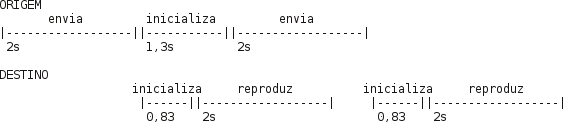
\includegraphics[scale=0.7]{./estrategia1.png}
 % ivamobile.jpg: 907x1385 pixel, 72dpi, 32.00x48.86 cm, bb=0 0 907 1385
\caption{Estratégia 1 - Linha do tempo}\label{figura_estrategia1}
\end{figure}

Uma análise rápida revela um atraso mínimo de 2,83 segundos, que é o tempo de captura do arquivo temporário na origem somado ao tempo de inicialização do MediaPlayer no destino. O autor reconhece que a técnica não serve para interação em tempo real, mas afirma que é o melhor resultado possível utilizando apenas as classes padrão do Android.

\subsection{Estratégia 2}
É a técnica implementada em~\cite{sipdroid}. Esta técnica utiliza a capacidade da classe MediaPlayer em reproduzir conteúdo ao vivo utilizando o protocolo RTSP.

\subsubsection{Na origem}
A classe MediaRecorder é utilizada para capturar vídeo. Os dados codificados são colocados diretamente em um socket local, que por sua vez é lido por um outro módulo que implementa o protocolo RTSP. Dessa forma os dados são enviados para o destino.

\subsubsection{No destino}
A classe MediaPlayer é inicializada e configurada para receber o conteúdo de um fluxo RTSP.

\subsubsection{Análise da estratégia}
O método resulta em um sistema de vídeo ao vivo, mas não em um sistema de interação em tempo real, pois a implementação do RTSP no Android não serve para tempo real. Tal afirmação foi comprovada através do seguinte experimento:

\begin{enumerate}
 \item Uma câmera foi conectada a um PC, tendo seu conteúdo capturado através do software VideoLAN Media Player (VLC)~\cite{VLC};
 \item O fluxo de dados proveniente do VLC foi direcionado para um servidor de streaming RTSP (Darwin Streaming Server~\cite{DSS}) especificado por um arquivo SDP (Session Description Protocol);
 \item O fluxo RTSP foi recebido em um smartphone Motorola Milestone (Android 2.0.1) utilizando a classe MediaPlayer.
\end{enumerate}

O atraso médio obtido durante o experimento foi de 10 segundos. Ao receber o mesmo fluxo em um VLC instalado em outro computador da mesma rede, o atraso foi de aproximadamente 1 segundo. Além do experimento proposto, também foi realizada uma comparação do RTSP do Android com o RTSP do VLC utilizando diversos links RTSP públicos na Internet. O mesmo resultado anterior foi verificado.

Comparado ao método anterior, nesta estratégia não ocorrem paradas na exibição. Porém, segundo os testes de desempenho realizados com a classe MediaPlayer, o atraso é maior do que no método anterior, devido ao baixo desempenho do RTSP utilizado juntamente com a classe MediaPlayer do Android.

\subsection{Estratégia 3}

Ao invés de utilizar a classe MediaRecorder para realizar a captura de áudio e vídeo, utiliza-se as classes Camera e AudioRecord. Ambas as classes permitem acesso direto aos dados não codificados. No entanto, não há nenhuma classe padrão do Android que codifique um fragmento de áudio ou vídeo a partir de dados não codificados, e quadros não codificados são grandes demais para serem transmitidos pela rede em tempo viável para vídeo interativo. 

Poderia ser implementado um codificador/decodificador em Java. No entanto, codificação e decodificação são processos que exigem um uso intensivo de CPU, ou seja, possuem um alto custo computacional, o que torna a solução inviável, uma vez que a implementação executaria sobre uma máquina virtual em um dispositivo com baixo poder computacional.

\subsection{Estratégia 4}

\subsubsection{Na origem}

Utilizar a função de foto da classe Camera, que retorna um quadro codificado em JPEG, e enviar cada quadro independentemente pela rede para o destino.

\subsubsection{No destino}

Receber cada quadro e exibi-lo com alguma classe padrão do Android que decodifique e exiba imagens JPEG.

\subsubsection{Análise da estratégia}

Codecs de vídeo são tipicamente mais eficazes do que codecs de imagens, visto que um vídeo é um conjunto de imagens relacionadas entre si, e a compressão leva em consideração a relação entre essas imagens. O codec JPEG apenas comprime uma imagem sem relacioná-la com nenhuma outra, portanto tem menos poder de compressão. Além disso, a função de foto do Android não foi projetada para este uso e é pouco eficiente. Um dos motivos é que quando a função foto é chamada, o preview do vídeo capturado é interrompido. Para tirar uma nova foto é preciso reiniciar o preview.

O método em si não foi testado pois, conforme justificado anteriormente, a estratégia é inviável independente da implementação. Outro problema da estratégia é não ter um correspondente para o áudio - somente o vídeo seria transmitido.

\subsection{Estratégia 5}
Como o Android possui código aberto, esta estratégia propõe copiar as bibliotecas nativas (C/C++) internas do sistema operacional que interagem com as classes MediaPlayer e MediaRecorder e com o hardware dos aparelhos, inserindo-as em um novo projeto compilável através da NDK. Desse modo teria-se acesso aos quadros codificados e decodificados pelo hardware e uma classe de transmissão de dados genéricos do Android poderia ser utilizada para realizar a transmissão e recepção dos dados multimídia. A implementação poderia ser organizada da seguinte forma:

\begin{itemize}
 \item Captura: câmera e microfone seriam acessados diretamente pelo código nativo, utilizando as bibliotecas internas do Android;
 \item Codificação e decodificação: em hardware, utilizando as bibliotecas internas do Android;
 \item Transmissão e recepção: alguma classe padrão do Android para transmissão e recepção de dados genéricos;
 \item Renderização: tela e alto falante seriam acessados diretamente pelo código nativo, utilizando as bibliotecas internas do Android.
\end{itemize}
 
Esta seria a solução mais eficiente possível, visto que todas as tarefas com alto custo computacional seriam realizadas em hardware, e os dados trafegariam pela rede comprimidos. Contudo, as bibliotecas nativas são dependentes de plataforma, ou seja, cada dispositivo tem particularidades de hardware que são generalizadas através da implementação de suas bibliotecas nativas. Utilizando a estratégia descrita, seria necessário manter diversas versões da mesma biblioteca, uma pra cada dispositivo. Por esse motivo, a manipulação de bibliotecas nativas internas do Android é desencorajado pelos desenvolvedores do Android. Além disso, essa solução é limitada à utilização dos codecs suportados por padrão pelos dispositivos.

\section{Solução adotada}

Pela análise acima pôde-se concluir que, até o momento, não é possível construir um sistema de interação por vídeo em tempo real utilizando apenas as classes padrão do Android. A solução proposta utiliza algumas das classes padrão do Android apresentadas, mas se baseia principalmente em implementações alternativas.

\subsection{Na origem}
\begin{enumerate}
 \item Utilizar a classe Camera para capturar os quadros de vídeo e instalar um callback que receba cada quadro não codificado obtido da captura. Com o auxilio dessa API, nós setamos os parâmetros de captura desejados (resolução, quadros/s, etc) e enviamos cada quadro capturado no formato YUV420SP (também conhecido como NV21, que é o único formato de captura suportado por todos os aparelhos Android) para o C++. A JNI é utilizada para passar os quadros do Java para o C++.
Um detalhe que convém citar é a utilização de Java reflection para que se possa chamar a função setPreviewCallbackWithBuffer em versões do Android anteriores a 2.2, quase dobrando a taxa de quadros em comparação ao método setPreviewCallback, visto que essa função evita que o garbage collector do Android interrompa o programa a cada quadro.
 \item Utilizar a classe AudioRecord para capturar os quadros de áudio, e obter os quadros não codificados da captura. Para isso desenvolvemos uma classe em Java que faz uso da classe AudioRecord, e captura o áudio do microfone. Cada quadro capturado é enviado ao C++ no formato RAW (PCM) com a utilização da JNI.
 \item Como o Android roda sobre um kernel Linux \todo{(FU et al., 2010)}, foi possível compilar o FFmpeg (que é uma solução que pode ser utilizada como uma biblioteca para codificar e decodificar vídeo em software \cite{ffmpeg} em C (com a NDK) adaptado para o Android. Desse modo, é possível codificar cada quadro de forma mais eficiente que em um codificador Java. No entanto, a implementação de diversos codecs de vídeo importantes fornecida pelo FFmpeg requer que o quadro decodificado de entrada esteja no formato YUV420P. Nesses casos, antes de codificar o quadro, é preciso convertê-lo de YUV420SP para YUV420P.
 \item Enviar os quadros codificados para o destino utilizando a implementação de sockets do C/C++. (Poderia-se passar os quadros codificados para o Java e enviá-los com alguma classe padrão do Android, mas a tarefa de passar os quadros com a JNI é custosa e complexa de ser implementada). Caso desejado, pode-se encapsular os pacotes respeitando qualquer protocolo específico (RTSP, SIP, RTMP, etc.) ou não utilizar nenhum protocolo.
\end{enumerate}

\subsection{No destino}
\begin{enumerate}
 \item Receber os quadros com a implementação de sockets do C/C++. (Igualmente poderia-se utilizar alguma classe padrão do Android, mas, pelo mesmo motivo citado no item anterior, não é o mais indicado). Pode-se criar um tratamento para o caso dos pacotes estarem de acordo com algum protocolo, como citado no item anterior.
 \item Decodificar os quadros de áudio e de vídeo com o FFmpeg em C/C++.
 \item Não há como acessar o alto falante e para renderizar os quadros de áudio diretamente do C++. A solução encontrada é passar os quadros de áudio decodificados para a classe AudioTrack utilizando a JNI. Desse modo, eles são reproduzidos. A API AudioTrack toca quadros de áudio que são entregues a ela no formato RAW (PCM). Para enviarmos os quadros de áudio do C++ para o Java, primeiramente tentamos chamar uma função Java a partir do C++ utilizando a JNI, passando como parâmetro o quadro, que seria a solução mais simples. No entanto, isso ativa o garbage collector a cada quadro, o que causa uma enorme queda no desempenho (100ms de interrupção por quadro, em média). Logo, essa ideia foi descartada. A alternativa que implementamos para evitar o garbage collector foi utilizar uma técnica da JNI um pouco mais trabalhosa. Em resumo, essa técnica consiste na criação de um array em Java que representa um quadro e de um array em C++ que também representa um quadro. Em seguida, com chamadas a algumas funções da JNI, associamos os dois arrays para a mesma posição de memória para que eles sejam tratados como se fossem um só. Assim, cada vez que se atualiza o array do C++ com os dados do novo quadro decodificado, essa atualização é automaticamente propagada ao array do Java, sem que seja feita nenhuma cópia e nenhuma alocação de memoria adicional, resultando na solução mais eficiente que encontramos para renderizar o áudio.
 \item Não há como acessar a tela para renderizar os quadros de vídeo diretamente do C++. Também não há alguma classe Java que receba como parâmetros quadros decodificados e renderize-os. A solução encontrada foi renderizar os quadros de vídeo com OpenGL ES \cite{opengl} em C++, desenhando um retângulo com as dimensões desejadas e aplicando o quadro de vídeo decodificado como textura RGB ao retângulo. No entanto, para que a renderização seja exibida na tela, é necessário que a função de renderização do C++ seja chamada de dentro do método onDrawFrame da classe GLSurfaceView.Renderer do Java e retorne para esse método a cada quadro. É importante citar que o OpenGL ES não renderiza quadros YUV. Desse modo, para os casos em que o FFmpeg apenas decodifica para YUV420P, é preciso convertê-lo de YUV420P para RGB. Outro detalhe importante, caso o quadro decodificado esteja numa resolução, e se queira renderizá-lo em outra, verificamos que realizando esse redimensionamento com o FFmpeg é mais lento que com o OpenGL ES. Ainda assim, caso a versão do OpenGL ES do aparelho utilizado seja a 1.0, o redimensionamento é feito em software. Caso seja 1.1 em diante, o redimensionamento é feito em hardware. Mais uma informação relevante: algumas versões do OpenGL ES suportam apenas texturas sobre retângulos de resolução cujas dimensões são potência de 2. Para poder desenhar o vídeo em qualquer resolução, criamos uma função que gera um retângulo com dimensões de potência de dois imediatamente maiores que as que irão ser utilizadas. Em seguida, a cada quadro, aplica-se a textura com qualquer dimensão sobre parte desse retângulo.
\end{enumerate}

\section{Análise da técnica e resultados}
\subsection{Teste 1}
Foi testada a decodificação e a exibição de um arquivo de vídeo local com a estratégia implementada em um dispositivo HTC Magic. Como resultado, para um vídeo de resolução 176x144, foram decodificados 227 quadros por segundo. A taxa de exibição obtida foi de 60 quadros por segundo (valor máximo suportado pelo aparelho).
\subsection{Teste 2}
Implementamos um aplicativo de videoconferência entre dispositivos móveis com a técnica apresentada. Para testar, realizamos uma conversa por vídeo com dois aparelhos Android caracterizados pela tabela~\ref{tabela_dispositivos}.
\begin{table}
\centering
\caption{Dispositivos utilizados nos testes}
\label{tabela_dispositivos}
\begin{tabular}{|p{1.5cm}|p{1.5cm}|p{1cm}|p{1.5cm}|p{1cm}|} \hline
Modelo&Processador&Versão do Android&Resolução máxima&Versão do OpenGL ES\\ \hline
Motorola Milestone A853&500MHz&2.0.1&480x854&1.0\\ \hline
Samsung Galaxy S GT-I9000B&1000MHz&2.1-update1&480x800&1.1\\
\hline\end{tabular}
\end{table}

Os parâmetros de codificação de vídeo utilizados no teste foram:
\begin{itemize}
 \item Resolução: 320x240
 \item Codec: MPEG-4
 \item Taxa de bits: 256Kbps
 \item GOP: 12
 \item Taxa de quadros: 15fps
\end{itemize}
Os parâmetros de codificação de áudio utilizados no teste foram:
\begin{itemize}
 \item Codec: MP2
 \item Taxa de bits: 64Kbps
 \item Frequência: 22050Hz
 \item Bits por amostra: 16
 \item Canais: 1
\end{itemize}

O vídeo era ampliado com o OpenGL ES para a resolução máxima do respectivo aparelho. A tabela~\ref{tabela_teste2} exibe os resultados do teste.

\begin{table}[htp]
\centering
\caption{Resultados do Teste 2}
\label{tabela_teste2}
\begin{tabular}{|p{1.5cm}|p{2.5cm}|p{1.2cm}|p{1.2cm}|} \hline
Dispositivo&Tipo de medida&Taxa de quadros&Tempo médio por quadro\\ \hline
Motorola&Captura do vídeo&15/s&1,16ms\\ \hline
Motorola&Captura do áudio&19/s&0,07ms\\ \hline
Samsung&Renderização do vídeo&14/s&2,88ms\\ \hline
Samsung&Renderização do áudio&18/s&19,62ms\\ \hline
Samsung&Captura do vídeo&15/s&0,72ms\\ \hline
Samsung&Captura do áudio&19/s&0,03ms\\ \hline
Motorola&Renderização do vídeo&15/s&16,03ms\\ \hline
Motorola&Renderização do áudio&19/s&33,39ms\\
\hline\end{tabular}
\end{table}

O atraso obtido ficou abaixo dos 400ms.

\subsection{Teste 3}
Realizamos uma transmissão de vídeo do Samsung para o Motorola (especificados na tabela~\ref{tabela_dispositivos}). Os parâmetros de codificação do áudio e do vídeo utilizados foram os mesmos do teste 2, porém com a taxa de quadros do vídeo igual a 30/s. A tabela~\ref{tabela_teste3} exibe os resultados do teste.

\begin{table}[htp]
\centering
\caption{Resultados do Teste 3}
\label{tabela_teste3}
\begin{tabular}{|p{1.5cm}|p{2.5cm}|p{1.2cm}|p{1.2cm}|} \hline
Dispositivo&Tipo de medida&Taxa de quadros&Tempo médio por quadro\\ \hline
Samsung&Captura do vídeo&30/s&0,58ms\\ \hline
Samsung&Captura do áudio&19/s&0,02ms\\ \hline
Motorola&Renderização do vídeo&29/s&12,77ms\\ \hline
Motorola&Renderização do áudio&18/s&24,24ms\\
\hline\end{tabular}
\end{table}

O atraso obtido foi inferior a 400ms.

\subsection{Teste 4}
O IVA é um sistema de videoconferências para computadores do tipo desktop~\cite{roesler_iva}. Seu foco principal é o ensino a distância. Utilizando a estratégia explicada neste trabalho, implementamos um aplicativo para Android que permite que o usuário do celular participe de videoconferências do IVA enviando seu vídeo e/ou visualizando o vídeo dos outros participantes.

Neste teste, o aplicativo Android recebeu um vídeo em tempo real codificado com MPEG-4 (vídeo) e MP2 (áudio) do IVA rodando em um desktop. Os parâmetros de codificação do vídeo foram: 1400 bit/s de taxa de codificação, 854x480 de resolução, 12 de GOP, codificado a 15 quadros por segundo. O áudio foi codificado a uma taxa de 128 bit/s. O Motorola (especificado na tabela~\ref{tabela_dispositivos}), rodando nosso aplicativo, recebeu e exibiu esta transmissão mantendo a taxa de 15 quadros por segundo. O áudio e o vídeo foram renderizados sincronizadamente e o atraso ficou abaixo dos 400ms. A figura~\ref{figura_eadcel} mostra o teste em execução.

\begin{figure}[htp]
 \centering
 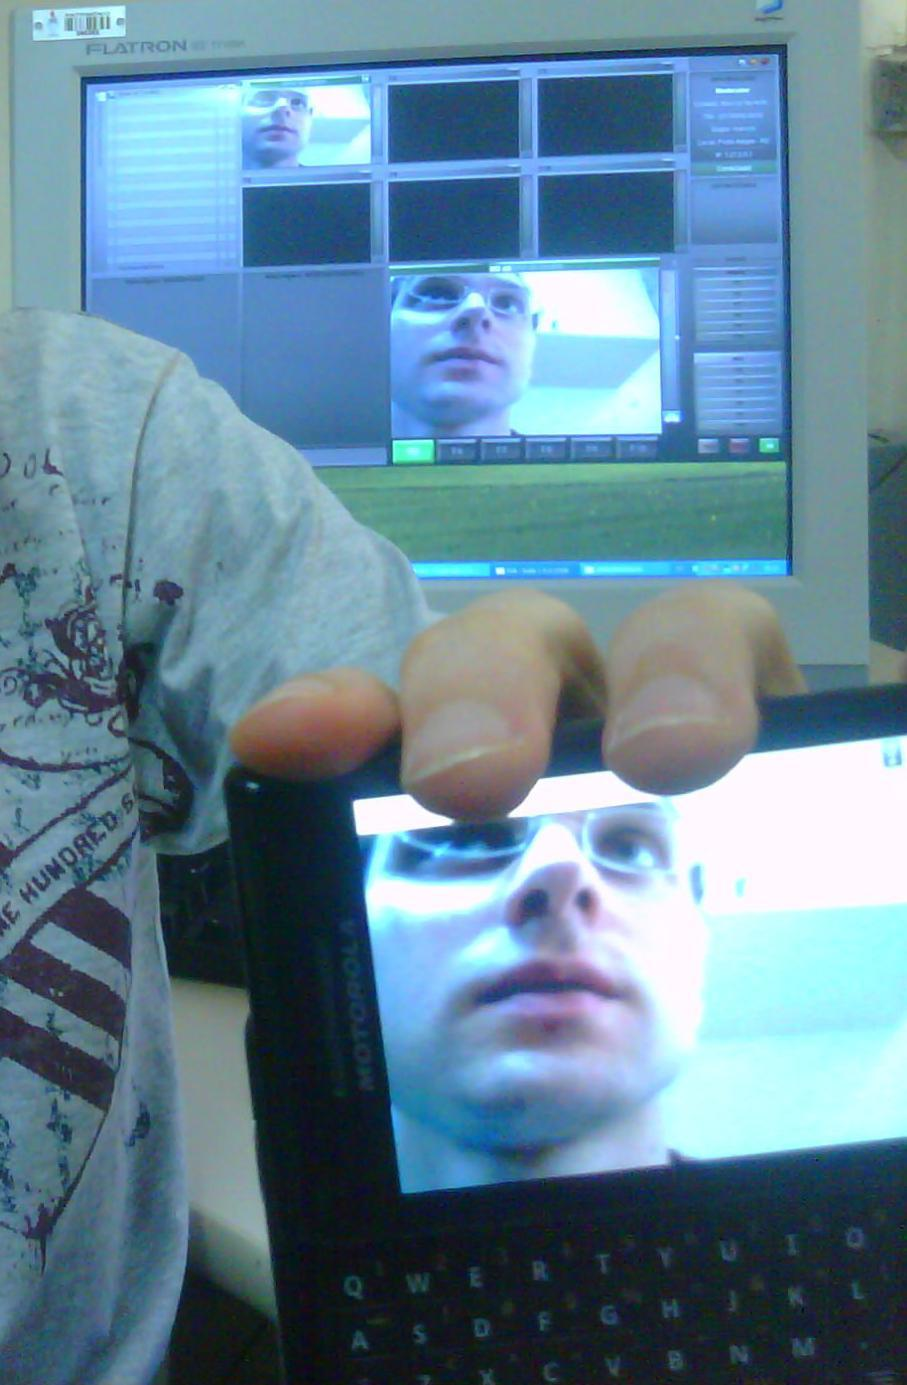
\includegraphics[scale=0.15]{./ivamobile.jpg}
 % ivamobile.jpg: 907x1385 pixel, 72dpi, 32.00x48.86 cm, bb=0 0 907 1385
\caption{Integração ao sistema IVA}\label{figura_eadcel}
\end{figure}

\subsection{Teste 5}
Também integramos nossa estratégia a um outro sistema de videoconferências já existente chamado BigBlueButton \cite{bbb}, que funcionava com suporte a vídeo apenas para desktops. Estamos desenvolvendo uma versão Android desse sistema, chamada de Mconf \cite{mconf}. Recebemos, no aplicativo Android Mconf (figura~\ref{figura_mconf}), um fluxo de vídeo do BigBlueButton gerado por um desktop. O codec de vídeo utilizado foi FLV1 (também conhecido como Sorenson H.263), a uma resolução de 320x240. O vídeo foi exibido ampliado na máxima resolução no Samsung e no Motorola especificados na tabela~\ref{tabela_dispositivos} e também em um tablet rodando Android. O atraso ficou abaixo dos 400ms.

\begin{figure}[htp]
 \centering
 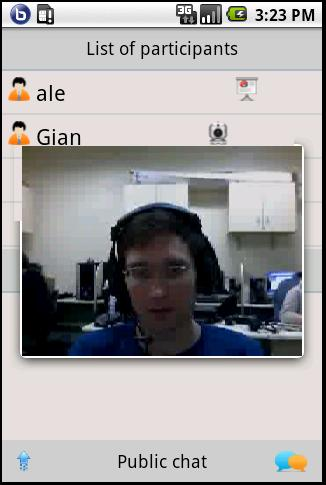
\includegraphics[scale=0.38]{./mconf.jpg}
 % ivamobile.jpg: 907x1385 pixel, 72dpi, 32.00x48.86 cm, bb=0 0 907 1385
\caption{Vídeo no Mconf: Integração ao sistema BigBlueButton}\label{figura_mconf}
\end{figure}

\section{Conclusão}

Este artigo apresenta uma solução para implementar transmissão de vídeo interativo em tempo real para Android, sendo consistente com versões do Android maiores ou iguais a 1.5. Os aspectos inovadores da estratégia são, principalmente, a codificação/decodificação de áudio e vídeo em software (com o FFmpeg compilado para o Android), a utilização da JNI para manipular os dados de áudio e de vídeo entre a camada nativa e a camada Java e a utilização de OpenGL ES para renderizar o vídeo. Todas essas escolhas são justificadas através de um estudo sobre as classes padrão do Android e suas limitações, seguida de uma comparação de estratégias propostas por trabalhos anteriores e seus resultados. Os testes da implementação da solução são apresentados, e seus resultados validam a utilização da técnica na implementação desse tipo de sistema.

Dentre os demais aspectos positivos da técnica, pode-se citar que ela é independente de protocolo. Em outras palavras, não há a necessidade de utilizar protocolos específicos, como o SIP, o RTSP e o RTMP, porém eles podem ser utilizados caso se deseje. Além disso, a solução não depende das classes MediaRecorder e MediaPlayer, o que a torna diferenciada, principalmente no que diz respeito a permitir a utilização de um grande número de codecs, até mesmo os não suportados pelo hardware do dispositivo. Adicionalmente, ao contrário dos trabalhos relacionados mencionados, nossa estratégia não apenas realiza codificação/decodificação e transmissão de áudio e vídeo, mas também faz essa transmissão em tempo real, permitindo o seu uso para conversas por vídeo e videoconferências.

\section{Trabalhos futuros}

Estamos desenvolvendo um framework que irá encapsular todas as partes complexas da implementação desta técnica. O framework permitirá que seja possível implementar aplicativos de interação por vídeo com a estratégia acima de modo simples e rápido, mas ao mesmo tempo oferecendo flexibilidade ao programador com relação a aspectos como, por exemplo, escolha dos codecs a serem utilizados e escolha da forma de transmissão/recepção dos dados codificados. Por exemplo, o programador, se desejar, poderá implementar seu próprio protocolo para transmissão, utilizar um protocolo padrão já existente, ou utilizar a transmissão fornecida pelo framework. Também será possível utilizar o framework para arquivos de vídeo locais que estão codificados com codecs ou formatos não suportados em hardware pelo Android, visto que o FFmpeg suporta, em software, um número muito grande de codecs.

%
% The following two commands are all you need in the
% initial runs of your .tex file to
% produce the bibliography for the citations in your paper.
\bibliographystyle{abbrv}
\bibliography{paper}  % sigproc.bib is the name of the Bibliography in this case
% You must have a proper ".bib" file
%  and remember to run:
% latex bibtex latex latex
% to resolve all references
%
% ACM needs 'a single self-contained file'!
%
\balancecolumns
% That's all folks!
\end{document}
